\documentclass[11pt]{article}

\usepackage[margin=1in]{geometry}
\usepackage{amsmath,amssymb,mathtools,bm}
\usepackage{booktabs}
\usepackage{microtype}
\usepackage[numbers,sort&compress]{natbib}
\usepackage{array}
\usepackage{longtable}
\usepackage{tabularx}
\usepackage{xcolor}
\usepackage{float}
\usepackage{tikz}
\usetikzlibrary{arrows.meta,positioning,calc}
\usepackage{hyperref}

\hypersetup{
  colorlinks=true,
  linkcolor=blue!55!black,
  citecolor=blue!55!black,
  urlcolor=blue!55!black,
}

\setlength{\parindent}{0pt}
\setlength{\parskip}{0.55em}
\renewcommand{\arraystretch}{1.16}

\newcommand{\R}{\mathbb{R}}
\newcommand{\Sym}{\operatorname{Sym}}
\newcolumntype{P}[1]{>{\raggedright\arraybackslash}p{#1}}
\newcolumntype{Y}{>{\raggedright\arraybackslash}X}

\title{Modern LLM Architecture\\
\large RNNs and Linear Attention: Time Evolution, Expansion, and Truncation}
\author{Haowu Duan}
\date{\today}

\begin{document}

\maketitle

This note uses the notation of recurrent neural networks to formulate numerical
time evolution, then derives linear attention from full softmax attention.  A
feature expansion turns attention into a recurrent state, and a finite
truncation makes that state practical.

% =====================================================================
\section{RNN refresher and linear attention from full attention}
% =====================================================================

A time-evolution differential equation is a natural setting for a recurrent
architecture.  For example, suppose a field $u(t,x)$ is carried at a constant
velocity $\bm c$.  This is the constant-velocity advection equation,
\begin{equation}
  \begin{split}
  \partial_t u(t,x)
  =-\bm{c}\mathbin{\cdot}\nabla u(t,x),
  \qquad x\in\Omega.
  \label{eq:advection-example}
  \end{split}
\end{equation}
More generally, write the evolution equation as
\begin{equation}
  \begin{split}
  \partial_t u(t,x)
  =\mathcal F[u(t,\,\cdot\,)](x),
  \qquad x\in\Omega.
  \label{eq:generic-time-evolution}
  \end{split}
\end{equation}
Here $\mathcal F$ denotes the right-hand-side operator.  It may contain
second derivatives such as $\nabla^2u$, derivatives of higher order such as
$\nabla^m u$ with $m>2$, transformations of the whole state such as
$\mathcal L\bm{u}(t)+\mathcal D\bm{x}(t)$ in
Equation~\eqref{eq:linear-driven-ode}, coefficient functions such as
$a(x)u(t,x)$ or
$\bm{b}(x)\mathbin{\cdot}\nabla u(t,x)$, or an integral term such as
$\int_\Omega K(x,x')u(t,x')\,dx'$.  Thus $\mathcal F$ can represent
essentially any evolution operator; it need not be local, linear, or even
differential.

After discretizing time, a one-step numerical method can be written as
\begin{equation}
  \begin{split}
  h_{n+1}(x)
  =h_n(x)+\Delta t\,\mathcal F[h_n](x)
  \equiv\mathcal T[h_n](x),
  \qquad
  h_n(\,\cdot\,)\equiv u(t_n,\,\cdot\,)\in\mathcal S.
  \label{eq:function-state-step}
  \end{split}
\end{equation}
The recurrent state is the entire function $h_n$, while the spatial coordinate
$x$ is the input at which that state is evaluated.  For the recurrent structure
considered here, $\mathcal F$ has no explicit time dependence and the step size
$\Delta t$ is fixed.  The induced map $\mathcal T$ is therefore identical at
every step, which is why neither operator carries a time subscript.  Repeatedly
applying the same map gives the recurrent structure.  We now make this
connection explicit in a model whose solution is known exactly.

\subsection{From an exactly solvable model to a recurrent step}

As an exactly solvable example, suppose the evolution is linear:
\begin{equation}
  \begin{split}
  \frac{d}{dt}\bm{u}(t)
  =\mathcal L\bm{u}(t)+\mathcal D\bm{x}(t),
  \qquad
  \bm{u}(0)=\bm{u}_0.
  \label{eq:linear-driven-ode}
  \end{split}
\end{equation}
This is a concrete linear example of
Equation~\eqref{eq:generic-time-evolution}.  Its exact solution is
\begin{equation}
  \begin{split}
  \bm{u}(t)
  =\mathcal A(t)\bm{u}_0+\mathcal B(t)[\bm{x}],
  \qquad
  \mathcal A(t)=e^{t\mathcal L},
  \qquad
  \mathcal B(t)[\bm{x}]
  =\int_0^t e^{(t-s)\mathcal L}\mathcal D\bm{x}(s)\,ds.
  \label{eq:linear-ode-solution}
  \end{split}
\end{equation}
$\mathcal A(t)$ advances the initial state when the input is zero.  It is the
exponential of the homogeneous operator $\mathcal L$.  The term
$\mathcal B(t)[\bm x]$ collects the effect of the input.  Differentiating its
integral with respect to the upper limit gives
\begin{equation}
  \begin{split}
  \frac{d}{dt}\mathcal B(t)[\bm{x}]
  =\mathcal D\bm{x}(t)+\mathcal L\mathcal B(t)[\bm{x}].
  \label{eq:forcing-integral-derivative}
  \end{split}
\end{equation}
Since $d\mathcal A/dt=\mathcal L\mathcal A$, the derivatives of the two terms
reproduce Equation~\eqref{eq:linear-driven-ode}.

Next discretize the differential equation.  With
$t_n=n\Delta t$, $\bm{h}_n\approx\bm{u}(t_n)$, and
$\bm{x}_n=\bm{x}(t_n)$, forward Euler gives
\begin{equation}
  \begin{split}
  \bm{h}_{n+1}
  =\bm{h}_n+\Delta t
    \left(\mathcal L\bm{h}_n+\mathcal D\bm{x}_n\right)
  =\mathcal A_{\Delta t}\bm{h}_n
   +\mathcal B_{\Delta t}\bm{x}_n
  =\mathcal T_{\Delta t}
   \begin{bmatrix}\bm{h}_n\\ \bm{x}_n\end{bmatrix},
  \label{eq:lti-rnn}
  \end{split}
\end{equation}
where
\begin{equation}
  \begin{split}
  \mathcal A_{\Delta t}=I+\Delta t\,\mathcal L,
  \qquad
  \mathcal B_{\Delta t}=\Delta t\,\mathcal D,
  \qquad
  \mathcal T_{\Delta t}
  =
  \begin{bmatrix}
    \mathcal A_{\Delta t} & \mathcal B_{\Delta t}
  \end{bmatrix}.
  \label{eq:discrete-transition}
  \end{split}
\end{equation}
Thus the one-step recurrent operator is the block row
$[\mathcal A_{\Delta t}\ \mathcal B_{\Delta t}]$.

Composing this same one-step transition $N$ times gives
\begin{equation}
  \begin{split}
  \bm{h}_N
  =
  \begin{bmatrix}
    \mathcal A_{\Delta t}^{N}
    & \mathcal A_{\Delta t}^{N-1}\mathcal B_{\Delta t}
    & \cdots
    & \mathcal B_{\Delta t}
  \end{bmatrix}
  \begin{bmatrix}
    \bm{h}_0\\
    \bm{x}_0\\
    \vdots\\
    \bm{x}_{N-1}
  \end{bmatrix}.
  \label{eq:discrete-evolution}
  \end{split}
\end{equation}
We now take $\Delta t\to0$ while keeping $t=N\Delta t$ fixed.  Then
\begin{equation}
  \begin{split}
  \mathcal A_{\Delta t}^{N}
  &=\left(I+\frac{t}{N}\mathcal L\right)^N
    \longrightarrow e^{t\mathcal L}
    =\mathcal A(t),\\
  \sum_{n=0}^{N-1}
    \mathcal A_{\Delta t}^{N-1-n}
    \mathcal B_{\Delta t}\bm{x}_n
  &\longrightarrow
    \int_0^t e^{(t-s)\mathcal L}\mathcal D\bm{x}(s)\,ds
    =\mathcal B(t)[\bm{x}].
  \label{eq:continuous-time-limit}
  \end{split}
\end{equation}
The repeated discrete transition therefore converges to the exact solution in
Equation~\eqref{eq:linear-ode-solution}.  This calculation shows the central
point: time discretization turns an evolution equation into repeated
applications of one shared transition.  In standard RNN notation, a learned
model replaces $\mathcal T_{\Delta t}$ by
\begin{equation}
  \begin{split}
  \bm{h}_t=\mathcal T_\theta(\bm{h}_{t-1},\bm{x}_t).
  \label{eq:shared-rnn}
  \end{split}
\end{equation}
Elman, LSTM, and GRU cells are three choices for this learned transition.

\subsubsection{Elman RNN}
The Elman RNN replaces the linear update by the trainable nonlinear step
\begin{equation}
  \begin{split}
  \bm{h}_t
  =\mathcal T_\theta[\bm{x}_t](\bm{h}_{t-1})
  =\tanh\!\left(
    \mathcal A\bm{h}_{t-1}+\mathcal B\bm{x}_t
  \right)\in\mathcal S.
  \label{eq:elman-cell}
  \end{split}
\end{equation}
The hyperbolic tangent acts componentwise.  In a differential-equation solver,
this cell is a learned nonlinear one-step map.
\begin{figure}[H]
\centering
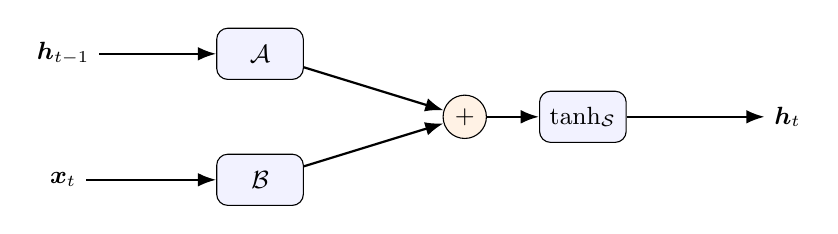
\begin{tikzpicture}[
  x=1cm,y=1cm,>=Latex,
  flow/.style={->,thick},
  map/.style={draw,rounded corners,minimum width=1.1cm,
    minimum height=0.65cm,fill=blue!5},
  op/.style={draw,circle,inner sep=1.5pt,minimum size=0.55cm,
    fill=orange!10},
  every node/.style={font=\small}
]
  \node (prev) at (0,1.1) {$\bm{h}_{t-1}$};
  \node[map] (A) at (2.5,1.1) {$\mathcal A$};
  \node (input) at (0,-0.5) {$\bm{x}_t$};
  \node[map] (B) at (2.5,-0.5) {$\mathcal B$};
  \node[op] (add) at (5.1,0.3) {$+$};
  \node[map] (nonlinearity) at (6.6,0.3) {$\tanh_{\mathcal S}$};
  \node (state) at (9.2,0.3) {$\bm{h}_t$};
  \draw[flow] (prev) -- (A);
  \draw[flow] (A) -- (add);
  \draw[flow] (input) -- (B);
  \draw[flow] (B) -- (add);
  \draw[flow] (add) -- (nonlinearity);
  \draw[flow] (nonlinearity) -- (state);
\end{tikzpicture}
\caption{The Elman transition combines the propagated state and injected input
before applying a componentwise nonlinearity.}
\label{fig:elman-cell}
\end{figure}
The weights are shared across steps, so the same nonlinear transition advances
the state throughout the sequence.  Elman networks were introduced for
next-step prediction and learning patterns in sequences
\citep{elman1990finding}.

\subsubsection{LSTM}
An Elman cell rewrites its entire state at every step.  Long short-term memory
(LSTM) adds a memory path that can preserve selected components across many
steps \citep{hochreiter1997lstm}.  Its recurrent state is the pair
\begin{equation}
  \begin{split}
  \bm{s}_t=
  \begin{bmatrix}
    \bm{c}_t\\
    \bm{h}_t
  \end{bmatrix},
  \qquad
  \bm{s}_t
  =\mathcal T_\theta[\bm{x}_t](\bm{s}_{t-1}).
  \end{split}
\end{equation}
The memory $\bm{c}_t$ and hidden state $\bm{h}_t$ are both internal to the
recurrent transition.  With
\begin{equation}
  \begin{split}
  \bm{z}_t=
  \begin{bmatrix}
    \bm{h}_{t-1}\\
    \bm{x}_t
  \end{bmatrix},
  \end{split}
\end{equation}
the update is
\begin{equation}
  \begin{split}
  \bm{f}_t
    &=\sigma(\mathcal W_f\bm{z}_t),\\
  \bm{i}_t
    &=\sigma(\mathcal W_i\bm{z}_t),\\
  \widetilde{\bm{c}}_t
    &=\tanh(\mathcal W_c\bm{z}_t),\\
  \bm{c}_t
    &=\bm{f}_t\odot\bm{c}_{t-1}
      +\bm{i}_t\odot\widetilde{\bm{c}}_t,\\
  \bm{o}_t
    &=\sigma(\mathcal W_o\bm{z}_t),\\
  \bm{h}_t
    &=\bm{o}_t\odot\tanh(\bm{c}_t).
  \label{eq:lstm-cell}
  \end{split}
\end{equation}
Here $\odot$ denotes componentwise multiplication.  The forget gate
$\bm f_t$ retains old memory, the input gate $\bm i_t$ writes the candidate,
and the output gate $\bm o_t$ controls which part of the updated memory is
exposed as $\bm h_t$.
\begin{figure}[H]
\centering
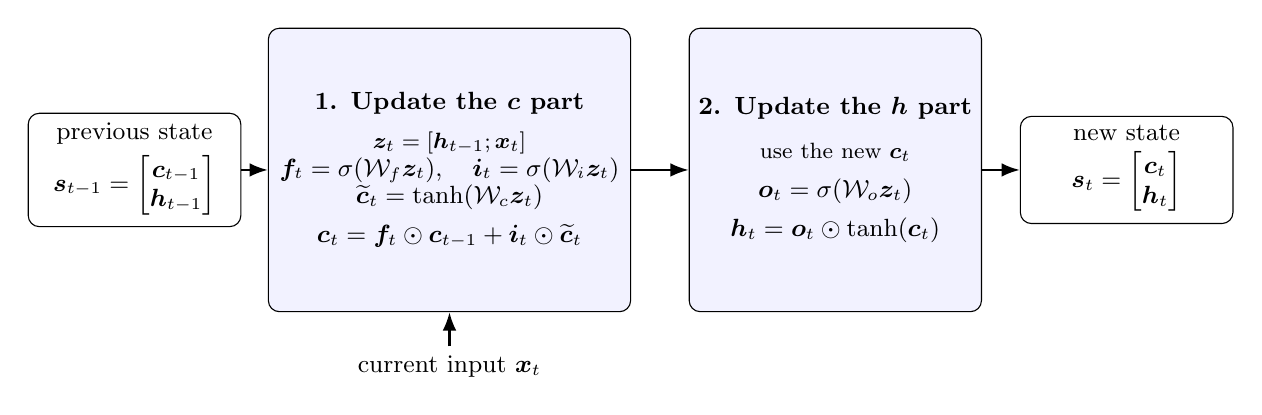
\begin{tikzpicture}[
  x=1cm,y=1cm,>=Latex,
  flow/.style={->,thick},
  state/.style={draw,rounded corners,minimum width=2.7cm,
    minimum height=1.35cm,fill=white,align=center},
  opbox/.style={draw,rounded corners,minimum height=3.6cm,
    fill=blue!5,align=center},
  every node/.style={font=\small}
]
  \node[state] (previous) at (0,0)
    {previous state\\[2pt]
     $\bm{s}_{t-1}=\begin{bmatrix}
        \bm{c}_{t-1}\\[-2pt]\bm{h}_{t-1}
      \end{bmatrix}$};
  \node[opbox,minimum width=4.6cm] (update-c) at (4,0)
    {\textbf{1. Update the $\bm{c}$ part}\\[3pt]
     \footnotesize
     $\bm{z}_t=[\bm{h}_{t-1};\bm{x}_t]$\\[-1pt]
     $\bm{f}_t=\sigma(\mathcal W_f\bm{z}_t),\quad
      \bm{i}_t=\sigma(\mathcal W_i\bm{z}_t)$\\[-1pt]
     $\widetilde{\bm{c}}_t=\tanh(\mathcal W_c\bm{z}_t)$\\[3pt]
     $\bm{c}_t=\bm{f}_t\odot\bm{c}_{t-1}
       +\bm{i}_t\odot\widetilde{\bm{c}}_t$};
  \node[opbox,minimum width=3.5cm] (update-h) at (8.9,0)
    {\textbf{2. Update the $\bm{h}$ part}\\[5pt]
     \footnotesize
     use the new $\bm{c}_t$\\[3pt]
     $\bm{o}_t=\sigma(\mathcal W_o\bm{z}_t)$\\[3pt]
     $\bm{h}_t=\bm{o}_t\odot\tanh(\bm{c}_t)$};
  \node[state] (next) at (12.6,0)
    {new state\\[2pt]
     $\bm{s}_t=\begin{bmatrix}
        \bm{c}_t\\[-2pt]\bm{h}_t
      \end{bmatrix}$};
  \node (input) at (4,-2.5) {current input $\bm{x}_t$};

  \draw[flow] (previous) -- (update-c);
  \draw[flow] (update-c) -- (update-h);
  \draw[flow] (update-h) -- (next);
  \draw[flow] (input) -- (update-c);
\end{tikzpicture}
\caption{The LSTM first updates the memory $\bm c_t$ and then exposes part of
that memory as $\bm h_t$.  Together they form the new recurrent state.}
\label{fig:lstm-cell}
\end{figure}
For a differential-equation solver, $\bm c_t$ is internal memory.  A readout from
$\bm h_t$ produces the numerical solution or physical observable.

\subsubsection{GRU}
The gated recurrent unit (GRU) keeps one persistent state vector rather than
the LSTM pair \citep{cho2014gru}.  It first constructs a candidate and then
mixes that candidate with the previous state.  With
$\bm{z}_t=[\bm{h}_{t-1};\bm{x}_t]$, one convention is
\begin{equation}
  \begin{split}
  \bm{r}_t
  &=\sigma(\mathcal W_r\bm{z}_t),\\
  \bm{u}_t
  &=\sigma(\mathcal W_u\bm{z}_t),\\
  \widetilde{\bm{h}}_t
  &=\tanh\!\left(
    \mathcal W_h[
      \bm{r}_t\odot\bm{h}_{t-1};\bm{x}_t
    ]\right),\\
  \bm{h}_t
  &=(\bm{1}-\bm{u}_t)\odot\bm{h}_{t-1}
    +\bm{u}_t\odot\widetilde{\bm{h}}_t.
  \label{eq:gru-cell}
  \end{split}
\end{equation}
The reset gate $\bm r_t$ controls how the old state enters the candidate, and
the update gate $\bm u_t$ interpolates componentwise between the old state and
that candidate.
\begin{figure}[H]
\centering
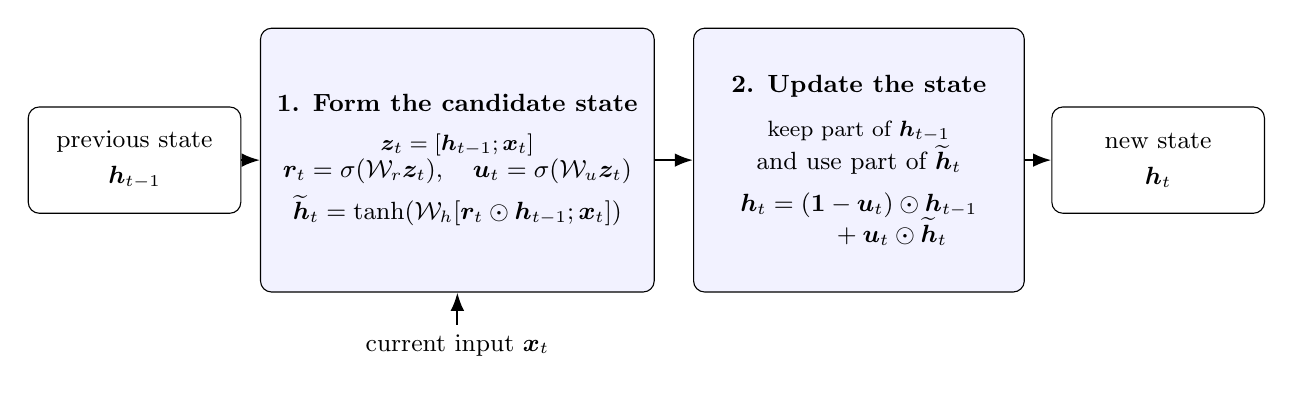
\begin{tikzpicture}[
  x=1cm,y=1cm,>=Latex,
  flow/.style={->,thick},
  state/.style={draw,rounded corners,minimum width=2.7cm,
    minimum height=1.35cm,fill=white,align=center},
  opbox/.style={draw,rounded corners,minimum height=3.35cm,
    fill=blue!5,align=center},
  every node/.style={font=\small}
]
  \node[state] (previous) at (0,0)
    {previous state\\[2pt]$\bm{h}_{t-1}$};
  \node[opbox,minimum width=5.0cm] (candidate) at (4.1,0)
    {\textbf{1. Form the candidate state}\\[3pt]
     \footnotesize
     $\bm{z}_t=[\bm{h}_{t-1};\bm{x}_t]$\\[-1pt]
     $\bm{r}_t=\sigma(\mathcal W_r\bm{z}_t),\quad
      \bm{u}_t=\sigma(\mathcal W_u\bm{z}_t)$\\[3pt]
     $\widetilde{\bm{h}}_t=\tanh\!\left(
       \mathcal W_h[\bm{r}_t\odot\bm{h}_{t-1};\bm{x}_t]
       \right)$};
  \node[opbox,minimum width=4.2cm] (update) at (9.2,0)
    {\textbf{2. Update the state}\\[5pt]
     \footnotesize
     keep part of $\bm{h}_{t-1}$\\[1pt]
     and use part of $\widetilde{\bm{h}}_t$\\[4pt]
     $\bm{h}_t=(\bm{1}-\bm{u}_t)\odot\bm{h}_{t-1}$\\[-1pt]
     $\phantom{\bm{h}_t={}}+
       \bm{u}_t\odot\widetilde{\bm{h}}_t$};
  \node[state] (next) at (13,0)
    {new state\\[2pt]$\bm{h}_t$};
  \node (input) at (4.1,-2.35) {current input $\bm{x}_t$};

  \draw[flow] (previous) -- (candidate);
  \draw[flow] (candidate) -- (update);
  \draw[flow] (update) -- (next);
  \draw[flow] (input) -- (candidate);
\end{tikzpicture}
\caption{The GRU forms a candidate state and then mixes it with the previous
state using the update gate.}
\label{fig:gru-cell}
\end{figure}

The linear recurrence, Elman cell, LSTM, and GRU differ in how they update the
state, but all process time steps sequentially and compress the relevant
history into a fixed-size state.  Full attention instead keeps previous token
states directly accessible.  We now ask when attention can be reorganized into
the same recurrent form.

\subsection{Attention as a transition kernel}

Suppose a sequence of length $S$ is processed by one attention head.  We
represent its input by $X\in\R^{S\times d_{\mathrm{model}}}$.  The head forms
\begin{equation}
  \begin{split}
  Q=XW_Q,\qquad K=XW_K,\qquad V=XW_V,
  \qquad Q,K,V\in\R^{S\times d_h}.
  \end{split}
\end{equation}
The $i$th rows $q_i$, $k_i$, and $v_i$ are the query, key, and value at
position $i$.  The index $i$ labels the output position, while $j$ labels a
position read by that output.

In causal attention, position $i$ can use only positions $j\leq i$.  Define
\begin{equation}
  \begin{split}
  \kappa(q_i,k_j)
  =\exp\!\left(\frac{q_i^{\mathsf T}k_j}{\sqrt{d_h}}\right),
  \qquad
  P_{ij}
  =\begin{cases}
    \frac{\kappa(q_i,k_j)}
         {\sum_{j'=1}^{i}\kappa(q_i,k_{j'})}, & j\leq i,\\[9pt]
    0, & j>i.
  \end{cases}
  \label{eq:attention-transition-kernel}
  \end{split}
\end{equation}
The head output is
\begin{equation}
  \begin{split}
  H_i
  =\sum_{j=1}^{S}P_{ij}v_j
  =\frac{\sum_{j=1}^{i}\kappa(q_i,k_j)v_j}
         {\sum_{j=1}^{i}\kappa(q_i,k_j)}
  \in\R^{d_h}.
  \label{eq:full-attention}
  \end{split}
\end{equation}
For fixed queries $Q$ and keys $K$, attention is the linear map $H=PV$ in the
values $V$, where $P$ is the lower-triangular transition kernel determined by
$Q$ and $K$.

\subsubsection{Full attention as an infinite-dimensional recurrent state}

To expose a recurrent structure, first expand the exponential kernel in
Equation~\eqref{eq:attention-transition-kernel}:
\begin{equation}
  \begin{split}
  \kappa(q,k)
  =\exp\!\left(\frac{q^{\mathsf T}k}{\sqrt{d_h}}\right)
  =\sum_{m=0}^{\infty}
    \frac{(q^{\mathsf T}k)^m}{m!\,d_h^{m/2}}.
  \label{eq:softmax-taylor}
  \end{split}
\end{equation}
For simplicity, let us truncate the kernel at second order:
\begin{equation}
  \begin{split}
  k_2(q,k)
  =1+\frac{q^{\mathsf T}k}{\sqrt{d_h}}
   +\frac{(q^{\mathsf T}k)^2}{2d_h}
  =\phi_2(q)^{\mathsf T}\phi_2(k).
  \label{eq:quadratic-kernel}
  \end{split}
\end{equation}
For example, when $d_h=2$, the two feature vectors are
\begin{equation}
  \begin{split}
    \phi_2(q)
    &=\left(
      1,
      \frac{q_1}{2^{1/4}},
      \frac{q_2}{2^{1/4}},
      \frac{q_1^2}{2},
      \frac{q_1q_2}{\sqrt{2}},
      \frac{q_2^2}{2}
    \right)^{\mathsf T},\\
    \phi_2(k)
    &=\left(
      1,
      \frac{k_1}{2^{1/4}},
      \frac{k_2}{2^{1/4}},
      \frac{k_1^2}{2},
      \frac{k_1k_2}{\sqrt{2}},
      \frac{k_2^2}{2}
    \right)^{\mathsf T}.
  \label{eq:quadratic-feature-vectors}
  \end{split}
\end{equation}
The kernel is symmetric in $q$ and $k$, so both arguments use the same feature
rule.  Permutation symmetry gives $q_1q_2=q_2q_1$ and $k_1k_2=k_2k_1$, so the
mixed monomial appears only once.  Its factor $1/\sqrt{2}$ accounts for the two
equal cross terms in $(q^{\mathsf T}k)^2$.  For general $d_h$, there is one
mixed coordinate $q_aq_b/\sqrt{d_h}$ for each pair $a<b$, and likewise for
$k$.  This example shows how each power of the dot product becomes a set of
feature coordinates.

Keeping every order gives an infinite feature vector $\Phi$ satisfying
\begin{equation}
  \begin{split}
  \Phi(q)^{\mathsf T}\Phi(k)
  =\sum_{m=0}^{\infty}
    \frac{(q^{\mathsf T}k)^m}{m!\,d_h^{m/2}}
  =\kappa(q,k).
  \label{eq:infinite-feature-map}
  \end{split}
\end{equation}

Substituting Equation~\eqref{eq:infinite-feature-map} into
Equation~\eqref{eq:full-attention} and reorganizing the sums gives
\begin{equation}
  \begin{split}
    H_i
    &=\frac{\sum_{j=1}^{i}
      \bigl[\Phi(q_i)^{\mathsf T}\Phi(k_j)\bigr]v_j}
      {\sum_{j=1}^{i}
      \Phi(q_i)^{\mathsf T}\Phi(k_j)}\\[3pt]
    &=\frac{
      \left[\sum_{j=1}^{i}\Phi(k_j)v_j^{\mathsf T}\right]^{\mathsf T}
      \Phi(q_i)}
      {\left[\sum_{j=1}^{i}\Phi(k_j)\right]^{\mathsf T}\Phi(q_i)}\\[3pt]
    &=\frac{F_i^{\mathsf T}\Phi(q_i)}
      {z_i^{\mathsf T}\Phi(q_i)},
  \label{eq:attention-recurrent-form}
  \end{split}
\end{equation}
where
\begin{equation}
  \begin{split}
  F_i=\sum_{j=1}^{i}\Phi(k_j)v_j^{\mathsf T},
  \qquad
  z_i=\sum_{j=1}^{i}\Phi(k_j).
  \end{split}
\end{equation}
Thus the recurrent state is the pair $(F_i,z_i)$.  When the next key--value
pair arrives, it updates as
\begin{equation}
  \begin{split}
  F_i=F_{i-1}+\Phi(k_i)v_i^{\mathsf T},
  \qquad
  z_i=z_{i-1}+\Phi(k_i),
  \qquad
  (F_0,z_0)=(0,0).
  \label{eq:moment-recurrence}
  \end{split}
\end{equation}
The update depends only on $(F_{i-1},z_{i-1})$ and the current pair $(k_i,v_i)$,
so it has exactly the recurrent structure introduced earlier.  If every
feature order is retained, Equation~\eqref{eq:full-attention} and this recurrent
form are identical.  The state is then infinite-dimensional and cannot be
stored.  In practice, linear attention keeps only finitely many feature
coordinates.  It is therefore a truncation of full attention in function
space.

We define $\Phi_p$ by retaining products of an input vector's components whose
exponents add to at most $p$.  These products are called monomials of total
degree at most $p$.  The resulting kernel is
\begin{equation}
  \begin{split}
  k_p(q,k)
  =\Phi_p(q)^{\mathsf T}\Phi_p(k)
  =\sum_{m=0}^{p}\frac{(q^{\mathsf T}k)^m}{m!\,d_h^{m/2}}.
  \label{eq:truncated-kernel}
  \end{split}
\end{equation}
Its feature dimension is
\begin{equation}
  \begin{split}
  r_p
  =\sum_{m=0}^{p}\binom{d_h+m-1}{m}
  =\binom{d_h+p}{p}.
  \label{eq:truncated-dimension}
  \end{split}
\end{equation}
The full feature vector is the limit $p\to\infty$, for which $r_p$ diverges,
so it cannot be stored in finite memory.  Even a low-order truncation can be
large at a realistic head dimension.  Llama 3.1 8B has model dimension 4096
and 32 attention heads, giving $d_h=128$ \citep{grattafiori2024llama3}.
For $p=2$, Equation~\eqref{eq:truncated-dimension} gives
\begin{equation}
  \begin{split}
  d_h=128,\qquad p=2
  \qquad\Longrightarrow\qquad
  r_2=\binom{128+2}{2}=8{,}385.
  \label{eq:llama-feature-dimension}
  \end{split}
\end{equation}
Thus even a second-order expansion requires 8{,}385 feature coordinates per
head.

The important advantage is that this state does not grow with the context
length.  Once $d_h$ and $p$ are fixed, $r_p(d_h+1)$ is fixed.  For one
full-attention head, define $M_{\mathrm{KV}}(S)$ as the number of scalar
entries in its key--value cache after $S$ tokens.  Each token contributes one
key and one value, both with $d_h$ entries, so
\begin{equation}
  \begin{split}
  M_{\mathrm{KV}}(S)&=2Sd_h=256S,\\
  M_{\mathrm{KV}}(8{,}192)&=2{,}097{,}152,\\
  M_{\mathrm{KV}}(131{,}072)&=33{,}554{,}432.
  \label{eq:llama-kv-growth}
  \end{split}
\end{equation}
Increasing the context from 8{,}192 to 131{,}072 tokens multiplies the full
key--value cache by sixteen.  The linear-attention state remains unchanged.
This independence from context length is the central advantage of linear
attention.

Replacing $\Phi$ by $\Phi_p$ gives the finite state and its recurrent update:
\begin{equation}
  \begin{split}
    F_i^{(p)}&=\sum_{j=1}^{i}\Phi_p(k_j)v_j^{\mathsf T},\\
    F_i^{(p)}&=F_{i-1}^{(p)}+\Phi_p(k_i)v_i^{\mathsf T},\\
    z_i^{(p)}&=\sum_{j=1}^{i}\Phi_p(k_j),\\
    z_i^{(p)}&=z_{i-1}^{(p)}+\Phi_p(k_i).
  \label{eq:finite-state}
  \end{split}
\end{equation}
This finite state is useful during autoregressive generation, when tokens are
produced one at a time.  Full attention must retain all previous keys and
values.  For a sequence of length $S$, its key--value cache contains
$2Sd_h$ numbers per head and therefore grows linearly with the sequence length.
The truncated recurrence retains only
$F_i^{(p)}\in\R^{r_p\times d_h}$ and $z_i^{(p)}\in\R^{r_p}$, for a total of
$r_p(d_h+1)$ numbers independent of $S$.  It uses less persistent memory once
$r_p(d_h+1)<2Sd_h$, and the advantage grows as the sequence becomes longer.
The same fixed state reduces the total processing cost from
$\mathcal{O}(S^2d_h)$ for full attention to $\mathcal{O}(Sr_pd_h)$ for linear
attention \citep{katharopoulos2020transformers}.  Equation~\eqref{eq:truncated-dimension}
also shows the tradeoff: increasing $p$ gives a richer feature map but can make
the recurrent state too large to retain this advantage.

{\small
\setlength{\parskip}{0pt}
\begin{thebibliography}{9}

\bibitem[Elman(1990)]{elman1990finding}
Elman, J.~L. (1990).
\newblock Finding structure in time.
\newblock \emph{Cognitive Science}, 14(2):179--211.

\bibitem[Hochreiter and Schmidhuber(1997)]{hochreiter1997lstm}
Hochreiter, S. and Schmidhuber, J. (1997).
\newblock Long short-term memory.
\newblock \emph{Neural Computation}, 9(8):1735--1780.

\bibitem[Cho et~al.(2014)]{cho2014gru}
Cho, K., van Merri\"enboer, B., G\"ul\c{c}ehre, C., Bahdanau, D., Bougares, F.,
Schwenk, H., and Bengio, Y. (2014).
\newblock Learning phrase representations using RNN encoder--decoder for
statistical machine translation.
\newblock In \emph{Proceedings of the 2014 Conference on Empirical Methods in
Natural Language Processing}, pages 1724--1734.

\bibitem[Grattafiori et~al.(2024)]{grattafiori2024llama3}
Grattafiori, A. et~al. (2024).
\newblock The Llama 3 herd of models.
\newblock \emph{arXiv preprint arXiv:2407.21783}.

\bibitem[Katharopoulos et~al.(2020)]{katharopoulos2020transformers}
Katharopoulos, A., Vyas, A., Pappas, N., and Fleuret, F. (2020).
\newblock Transformers are RNNs: Fast autoregressive Transformers with linear
attention.
\newblock In \emph{Proceedings of the 37th International Conference on Machine
Learning}.

\end{thebibliography}
}

\end{document}
